\documentclass[11pt]{amsart}
\usepackage[margin=1in,top=0.7in]{geometry}
\usepackage{enumitem}
\usepackage{graphicx}
\usepackage{hyperref}

\newcommand{\R}{\mathbb{R}}
\newcommand{\Q}{\mathbb{Q}}
\newcommand{\vr}[2]{\mathrm{VR}(#1;#2)}

\title{Research Proposal}
\author{Joshua Mirth}
\date{\today}

%\linespread{1.8}

\begin{document}

\maketitle 
%I am pleased to announce that The Mathematics Department will be able to support up to two graduate research fellowships during the summer of 2018. These fellowships will provide a \$4080.00 stipend.  An application should include a research proposal, a letter of support from the student’s advisor and a predicted timeline to graduation.  The research proposal should be written at a level understandable by a mathematician with expertise in a different area and should provide a context for the work that is proposed during the summer. The research proposal should be no more than three pages long.  All application materials should be submitted electronically to Bryan Elder by March 16 2018.  

\section{Current and Previous Work}

In the fall of 2017 I completed a masters thesis on Metric Thickenings of Euclidean submanifolds.
%This was an extension of earlier work by my advisor and his collaborators \cite{AdamaszekMetricreconstructionoptimal2017}.
The main result was a homotopy equivalence between manifolds embedded in Euclidean space and their metric thickenings (an object introduced in \cite{AdamaszekMetricreconstructionoptimal2017} and of interest in computational topology).
As topological data analysis is usually done in a high-dimensional Euclidean setting, there is practical merit in having theoretical results in that context. 
Moreover, the proof of this result exploited the geometry of Euclidean space, demonstrating techniques that were not available in earlier work such as \cite{AdamaszekMetricreconstructionoptimal2017} (which gave an analogous result for Riemannian manifolds).
This work has been submitted and can be found at \href{https://arxiv.org/abs/1709.02492}{arXiv:1709.02492} \cite{AdamsMetricthickeningsEuclidean2017}.
%The primary development from my thesis was to extend their results into the context of embedded manifolds with the Euclidean metric rather than intrinsic Riemannian one \cite{AdamsMetricthickeningsEuclidean2017}.
%Though the results are quite analogous, many of the methods were distinctly different.
%In particular, the proof of the main result (a homotopy equivalence between two spaces) exploited the geometry of Euclidean space in ways that were not available in the context of the earlier work.
%Also, topological data analysis is usually done in a high-dimensional Euclidean setting, so there is practical merit in having theoretical results in that context.
%(The classical result here is \cite{NiyogiFindingHomologySubmanifolds2008}.)

My current work involves two separate projects.
One is a collaborative effort as part of the Pattern Analysis Lab to define and compute a persistent homology fractal dimension.
Second, expanding on the directions explored for my masters, I am now investigating the homotopy groups of the metric thickenings of geodesic spaces, generalizing \cite{GasparovicCompleteCharacterization1Dimensional2017} and \cite{Virk1DimensionalIntrinsicPersistence2017}. 
I expect both of these projects to be substantively completed by the end of the spring of 2018.

\section{Proposed Future Work}

A longer term project with relevance to my dissertation is presented below.
The main idea is to develop a Morse theory that is applicable to filtered simplicial complexes, such as the \v{C}ech and Vietoris--Rips complexes used in applied topology. 
A summer graduate research fellowship would allow me to make significant progress in this direction, as well provide the time and flexibility to attend the Theory and Foundations of TGDA workshop at the Ohio State University and the Tutorial on Multiparameter Persistence, Computation, and Applications at the University of Minnesota IMA, both of which have direct bearing on this research.

\subsection{A brief history of Morse Theory}

Morse theory played a major role in the development of differential topology from the 1930s onward.
The idea is simple: given a smooth manifold $M$, there is a generic class of smooth functions $f \colon M \to \R$, called Morse functions.
The critical points of such function (that is, the points for which $\nabla f = 0$) determine the topological structure of $M$.  
Specifically, there are two fundamental lemmas:
\begin{enumerate}[label=(\alph*)]
\item If $[a,b]$ contains no critical values of $f$, then $f^{-1}(-\infty,a]$ and $f^{-1}(-\infty,b]$ are homeomorphic, and
\item if $x$ is a critical point of $f$ of index $k$, then $f^{-1}(-\infty,x+\epsilon]$ is homotopy equivalent to $f^{-1}(-\infty,x-\epsilon]$ with a $k$-cell glued on.
\end{enumerate}
The classical example of the height function on the torus, due to \cite{MilnorMorseTheory1963}, is show in Figure \ref{fig:torus}.
Stephen Smale's proof of the $h$-cobordism theorem, and consequently the generalized Poincar\'{e} conjecture, can be considered as extensions of this theory \cite{MilnorLectureshCobordismTheorem1965}.

\begin{figure}[h]
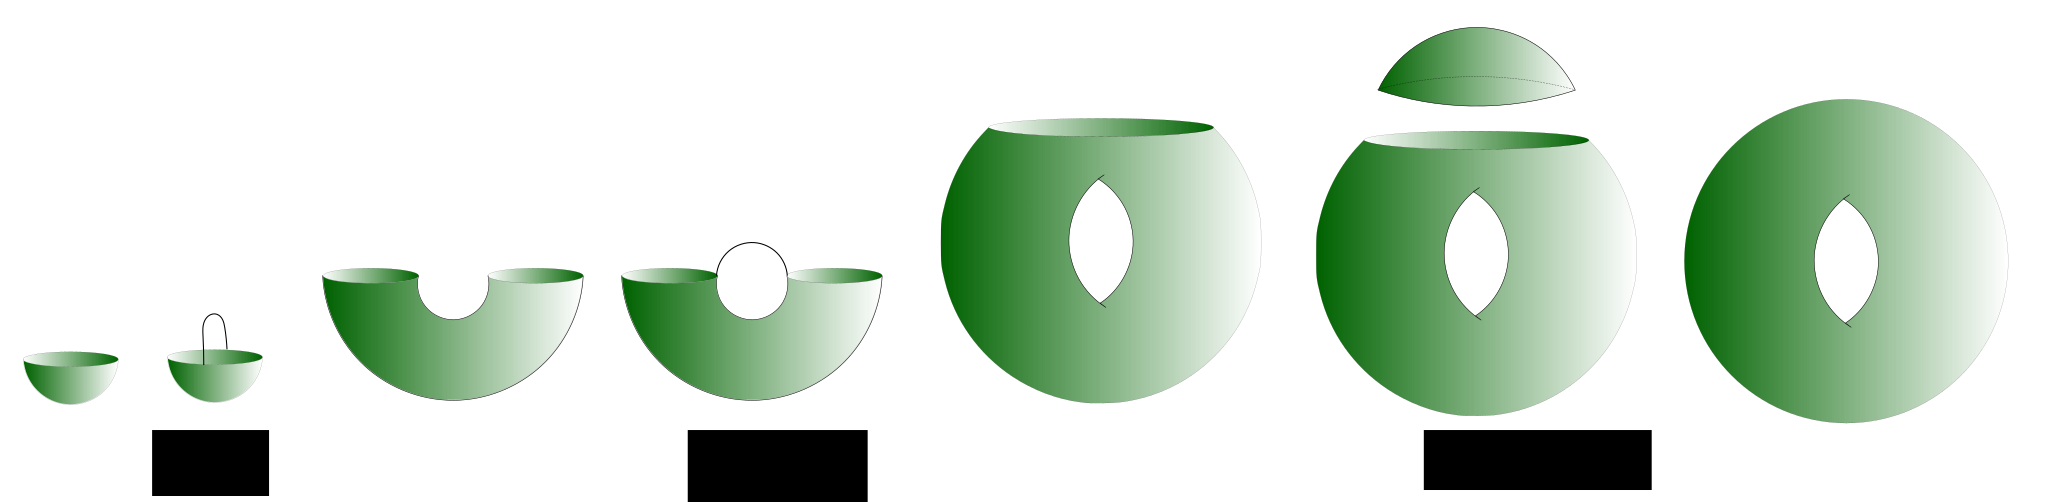
\includegraphics[width=5in]{morse_torus.png}
\caption{At an index-$k$ critical point, the topological structure changes by the gluing on of a $k$-cell.} 
\label{fig:torus}
\end{figure}

The sublevel sets $f^{-1}(-\infty,r]$ of a Morse function give a filtration of $M$ indexed by the real numbers, in other words, for $r < r'$ we have $f^{-1}(-\infty,r] \subseteq f^{-1}(-\infty,r']$.
Persistent homology, an underlying theory of applied topology, is based on a generalization of this idea \cite{EdelsbrunnerComputationalTopologyIntroduction2008}.
Persistence takes as input a filtered sequence of topological spaces and analyzes how the structure of the space varies with the filtration.
Of particular interest are the distances between the filtration values at which the topology changes (i.e.\ the length of the barcodes).
In data analysis long intervals are often presumed to represent real features of the data while short ones signify sampling noise.

One source of such a filtration is to cover a metric space, $X$, by a union of balls of radius $r$.
Varying the radius gives a filtration of spaces.
This can be converted into combinatorial data, making computations feasible, by forming a simplicial complex with vertices corresponding to the balls and higher-dimensional simplices corresponding to $n$-fold intersections of balls.
The Nerve Theorem says that this complex has the same homotopy type as the union of the balls, and so for small $r$ provides a good approximation of the topology of $X$.
% Should I name it?

Discrete Morse theory, due to Robin Forman \cite{FormanMorseTheoryCell1998}, which considers critical simplices in a simplicial complex $K$.
A Morse function is a map $f \colon K \to \Q$ with certain matching constraints.
Simplices on which $f$ is injective are the critical simplices, and their dimension corresponds to the index of critical points in the classical theory.
Perhaps surprisingly, given that none of the machinery of differential geometry is available, this theory replicates most of the major results on smooth manifolds \cite{BenedettiSmoothingdiscreteMorse2012}.

\subsection{Problem Statement} 
This leads to the crux of the matter: in applied topology one would desire to identify not only critical simplices, but critical \emph{scale parameters}.
Consider for instance the simplicial complex formed on six equally spaced points around a circle of circumference one using the Vietoris--Rips construction (a minor variant of the construction described in the preceding paragraph).
For scale parameters (in this case, radii) less than $1/3$, the simplicial complex is homotopy equivalent to a circle, and exactly one of the $1$-simplices is critical in the sense of \cite{FormanMorseTheoryCell1998} (see Figure \ref{fig:vrcircle}).
At $r = 1/3$, two simplices appear which fill in the center of the circle, resulting in the homotopy-type of a $2$-sphere (see \cite{AdamaszekVietorisRipsComplexes}).
At this fixed $r$, the established discrete Morse theory detects that the only critical simplex is one of the enclosing $2$-simplices.
However, this theory is agnostic to the filtration data; there is no \emph{a priori} method to determine that $r = 1/3$ should be a scale parameter at which the homotopy-type changes.
I seek to develop a Morse theory in which the critical data is both the simplices and the scale parameter.

\begin{figure}[h]
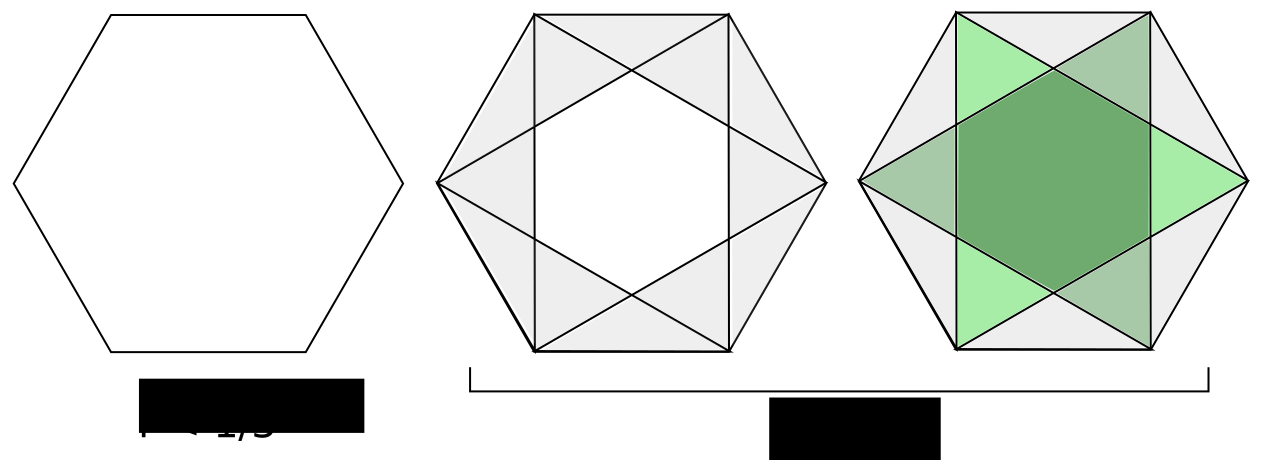
\includegraphics[width=3in]{rips_critical.png}
\caption{Vietoris--Rips complex with $r < 1/3$ (left). At $r = 1/3$, $2$-simplices form around the perimeter (center) and across the middle (right), forming an enclosed polygon homotopy equivalent to a sphere.}
\label{fig:vrcircle}
\end{figure}

The benefits of such a theory are two-fold. 
Topological data analysis often tries to identify an underlying manifold from a simplicial complex built on a data set.
Unfortunately, the structure of simplicial complexes built on manifolds is largely unknown (except that for some range of scale parameters it is the same as the manifold itself).
Morse theory would provide a natural tool to address this question. %especially since explicit computation of the topology of an infinite simplicial complex is difficult.
This might also address a longstanding conjecture of Jean-Claude Hausmann that the dimension up to which all homotopy groups of the Vietoris--Rips complex of a manifold vanish is a non-decreasing function of the scale parameter \cite{HausmannVietorisRipsComplexes1995}.

%Second, an outstanding problem in persistence theory is that the structure of persistence modules is only well-behaved when (co)homology is computed with coefficients in a field.
%However, it is desirable (e.g.\ by the universal coefficient theorem) to compute persistence with integer coefficients.
%This is understood but only when the index set of the filtration is discrete \cite{?}
%A sufficiently robust Morse Theory could reduce persistence computations from a continuum to a discrete set of critical values, possibly side-stepping this difficulty.

Second, persistent homology is computationally expensive.
Using the similarity between simplicial complexes and certain algebraic chain complexes, Sk\"{o}ldberg and others developed a purely algebraic Morse Theory \cite{SkoldbergMorsetheoryalgebraic2006}.
This has been used in applied topology, for example in \cite{CurryDiscreteMorsetheory2016} where the authors used algebraic Morse theory to produce more efficient algorithms for the computation of sheaf cohomology.
A better understanding of the structure of filtered simplicial complexes through Morse theory has potential to lead to improved algorithms for persistent homology computations.

\subsection{Proposed Approach}
Given the above reasons to develop a Morse theory for Vietoris--Rips complexes, I propose to work on some first steps in the development of such a theory.
The key components are a notion of Morse functions on a Vietoris--Rips complex, $\vr{X}{r}$, a definition of critical point, and the correct idea of index for critical points.
Following are some proposed definitions.

First, for $r < r'$ there is a canonical inclusion $\vr{X}{r}$ into $\vr{X}{r'}$.
All scale parameters can be encoded by considering $\vr{X}{\infty}$, the maximum complex in this system of inclusions.%, or for an infinite index set the colimit thereof.
A Morse function $f \colon \vr{X}{\infty} \to \R$ would be given by the map sending each point to the minimum diameter simplex in which it is contained.
The sublevel set $f^{-1}(-\infty,r)$ is then precisely equal to $\vr{X}{r}$.
A simplex of diameter $r$ will be called \emph{filtration maximal} if it is maximal under inclusion in $\vr{X}{r}$.
Denote the set of barycenters of filtration maximal simplices by $B$.
For known examples, $B$ is a disjoint union of manifolds, and $f$ restricted to $B$ appears to be a Morse function (in the classical sense) on each connected component.
Thus, define a simplex to be critical if its barycenter is a critical point of $f\vert_B$.
Define the index of the critical $k$-simplex $\sigma$ with barycenter $b$ to be $k + \mathrm{index}(b)$ (where index is meant in the classical sense).

I then conjecture that both Morse lemmas hold; namely
\begin{enumerate}[label=(\alph*)]
\item if there is no critical value in $[r,r']$, then $\vr{X}{r} \sim \vr{X}{r'}$, where the equivalence is at least as strong as homotopy equivalence, and
\item at a critical point of index $i$, the homotopy type changes by the gluing on of an $i$-cell.
\end{enumerate}
These definitions may require modification, but the above are known to hold as is for the circle, more generally the $n$-sphere, and for ellipses of small eccentricity.

\bibliographystyle{plain}
\bibliography{GRA_Application}

\end{document}
